\section{Introduction}

\STANDARD{\insertsection}
{ 
 \textbf{Case Describtion}\\
The main focus of this project is to use the Arduino Portenta H7 IMU to recognize gait patterns.\\
\bigskip
The fundamental objective of this gait pattern recognition is to anticipate injuries to the human body's lowest (the foot).

\bigskip

\textbf{Main Challenges of entire process. }\\
\bigskip
\begin{itemize}
    \item 1. To recognize the walking pattern using an accelerometer-equipped Arduino Portenta H7 IMU sensor.
    \item 2. Identification of speed based on gait terminology.
    \item 3. To analyse feet movement and classifying other aspect of foot's movement.
\end{itemize}
}

\section{Positioning the Analytics in front of Existing Solution}
\STANDARD{\insertsection}
{ 
IMU-based gait recognition using convolutional neural networks and multi-sensor fusion
    \begin{figure}[h]
    \centering
    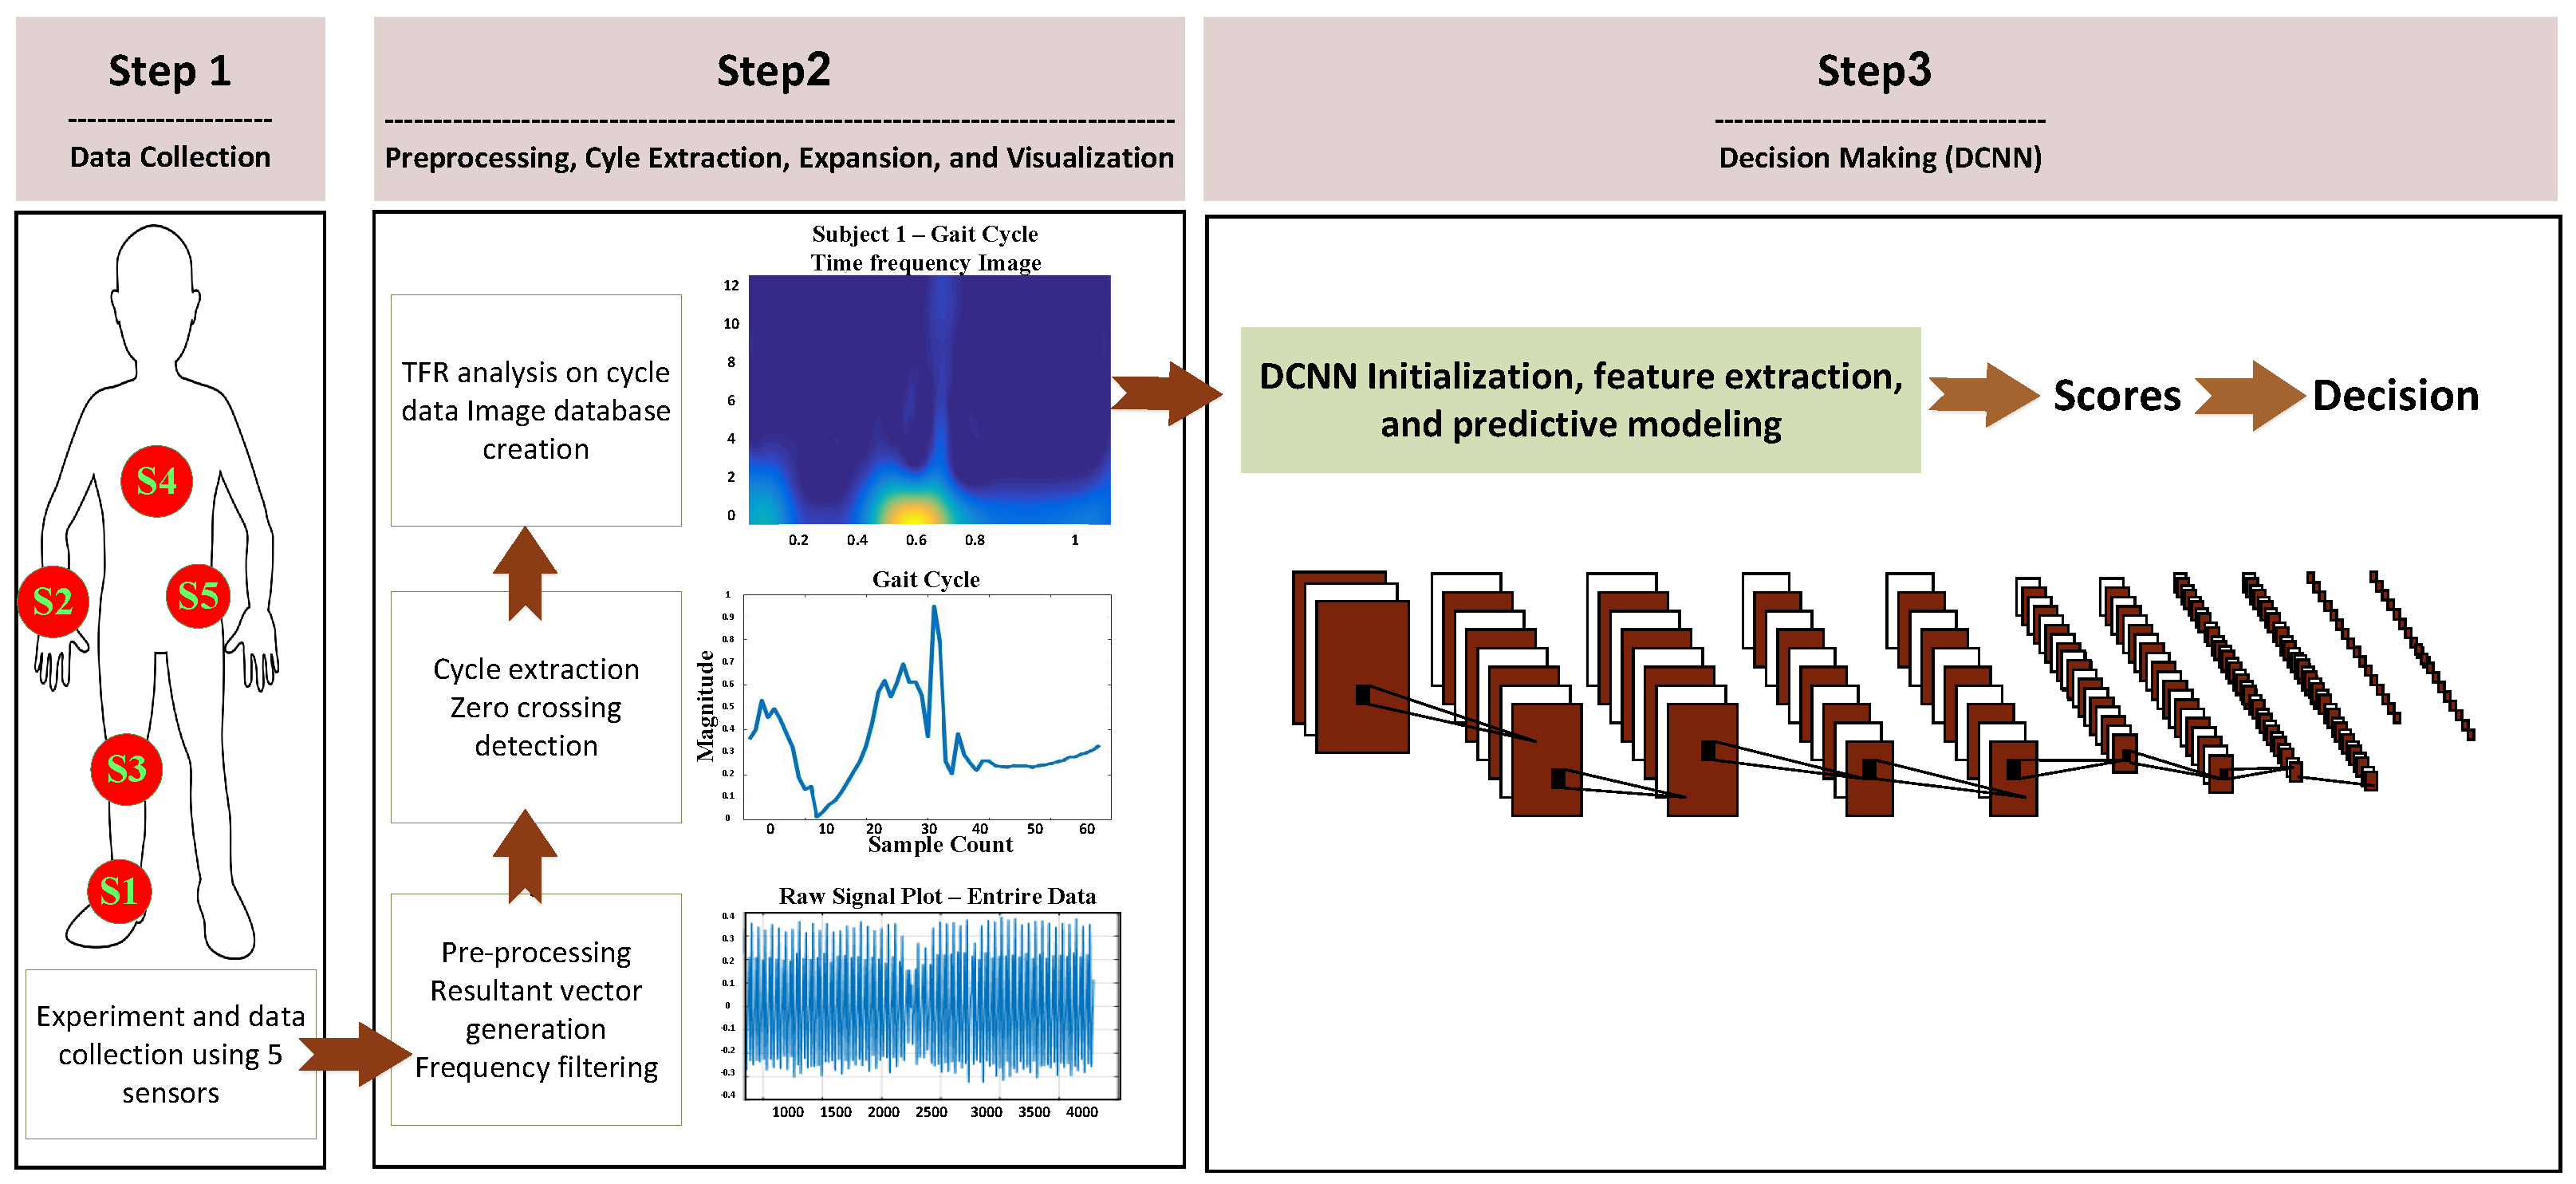
\includegraphics[scale=0.08]{img/The overview of our existing system for Human Gait Identification.png}
    \caption{The overview of existing system source: \cite{Dehzangi2017}}
    \label{fig:The overview of existing system for Human Gait Identification}
\end{figure}
    
}

\section{Identify the Application Sector for your Analytic}
\STANDARD{\insertsection}
{ 
BTS Bioengineering's app uses functional assessment tests to prevent injuries and identify optimal rehabilitation protocols. 
  \begin{figure}
    \centering
    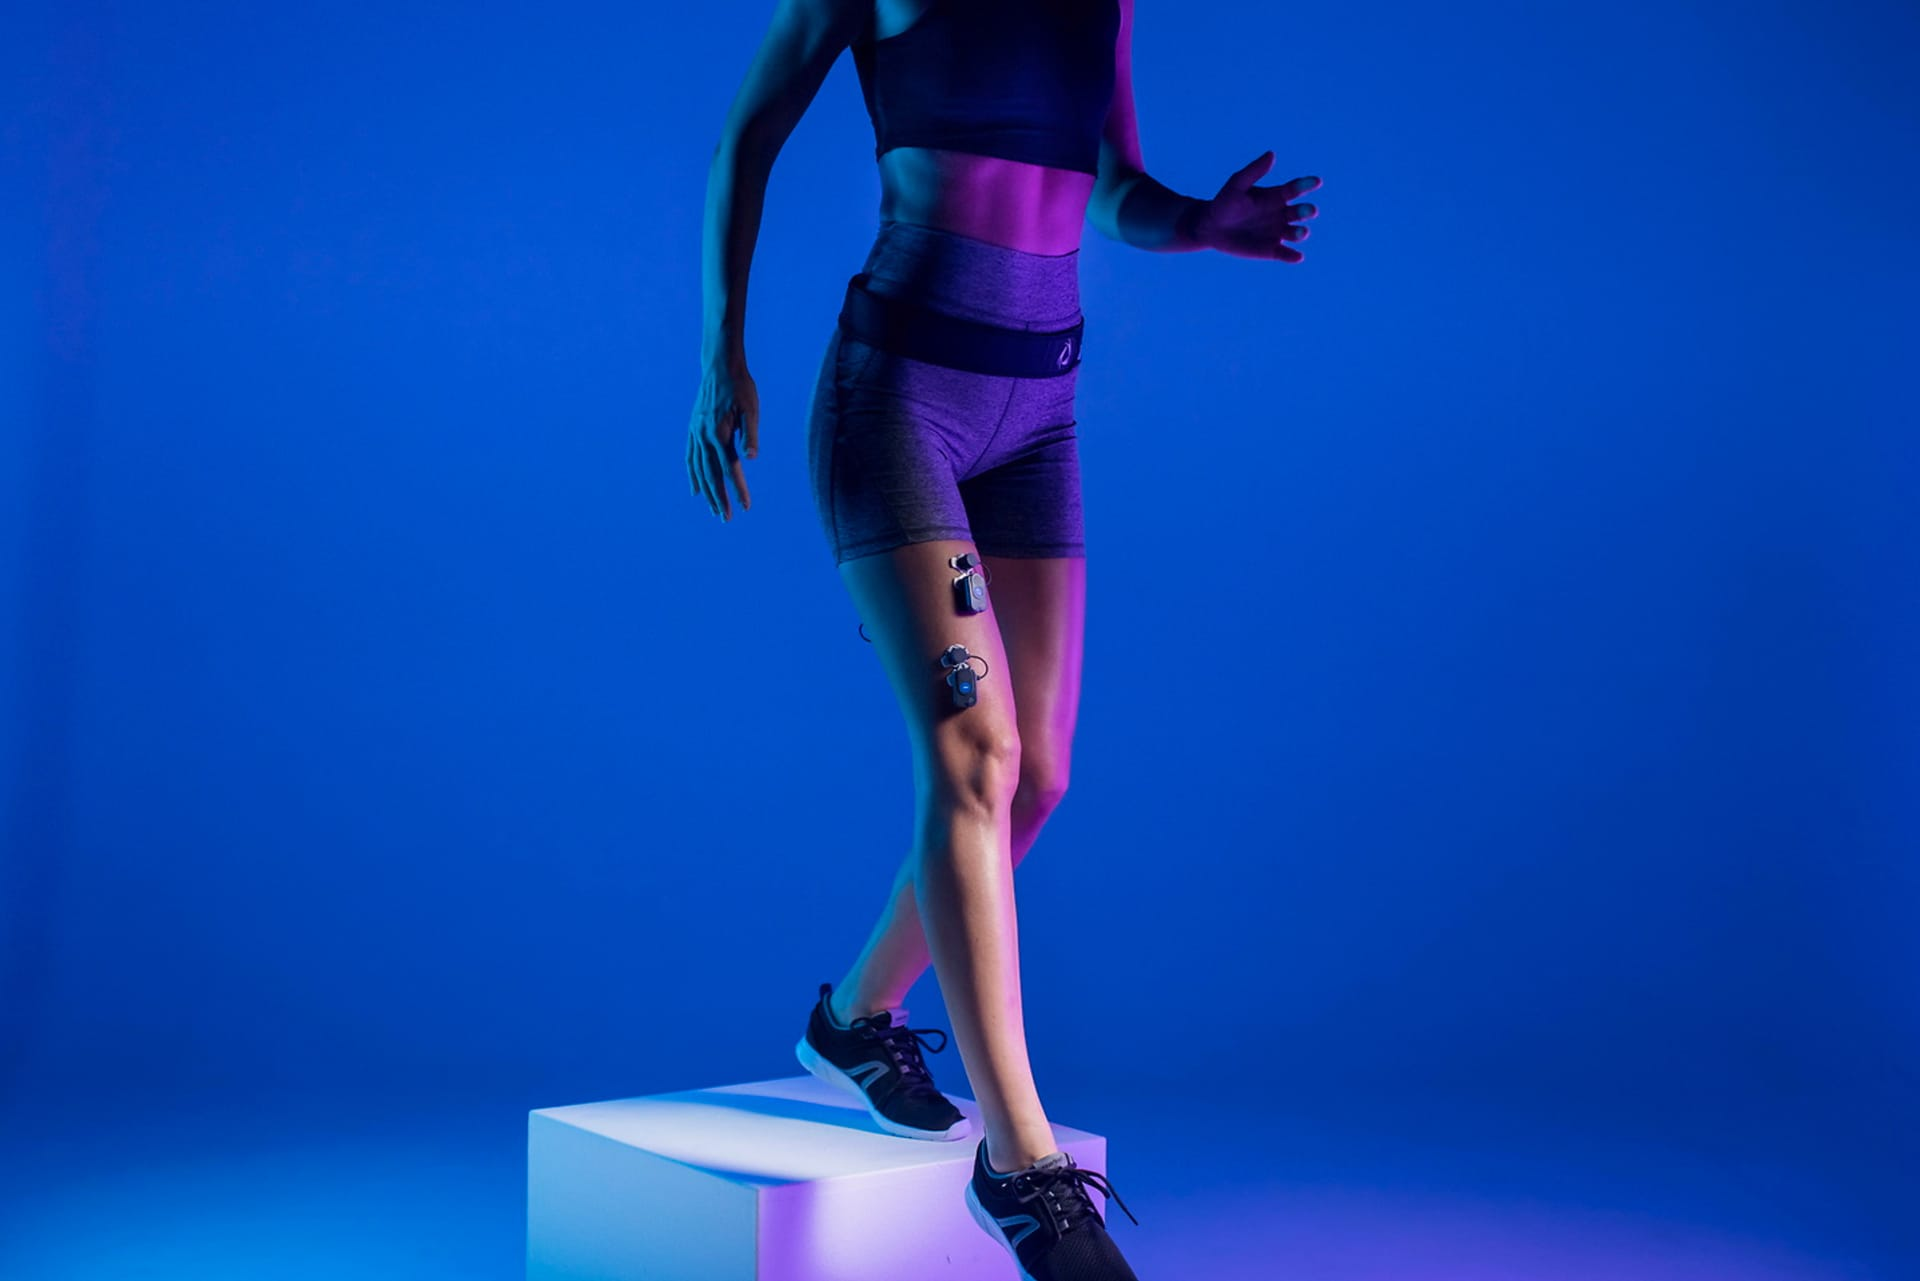
\includegraphics[scale=0.1]{img/Injury prevention and return to play.jpeg}
    \caption{Injury prevention and return to play application source: \cite{BTS_Injury_prevention2022}}
    \label{fig:Injury prevention and return to play}
\end{figure}
}

\section{What is your analytic doing}
\STANDARD{\insertsection}
{
    Our project improves the financial viability and effectiveness of an accelerometer-based gait analysis system. The system measures sagittal rotation in the mediolateral axis and identifies four essential walking events: Heel-Strike (HS), Toe-Strike (TS), Heel-Off (HO), and Toe-Off (TO). These events will distinguish gait patterns. Two parts explain our analytics.
    
    \bigskip
    \textbf{1. Diagnosis of gait patterns.}
    
    \begin{itemize}
    \item   i. Data-Preparation.
    \item  ii. Gait Cycle Extraction.
    \end{itemize}
    \textbf{2. Differentiate of gait pattern.}
    \begin{itemize}
    \item   i. Recurrent Neural Networks (RNN) Initialization.
    \item  ii. Feature extraction.
    \item iii. Predictive of injury modelling.
    \end{itemize}
}

\section{Position of Analysis in Standard Reference Architecture}
\STANDARD{\insertsection}
{
\textbf{The Reference Architecture Model Industrie 4.0 (RAMI 4.0)} 
\begin{figure}[ht]
    \centering
    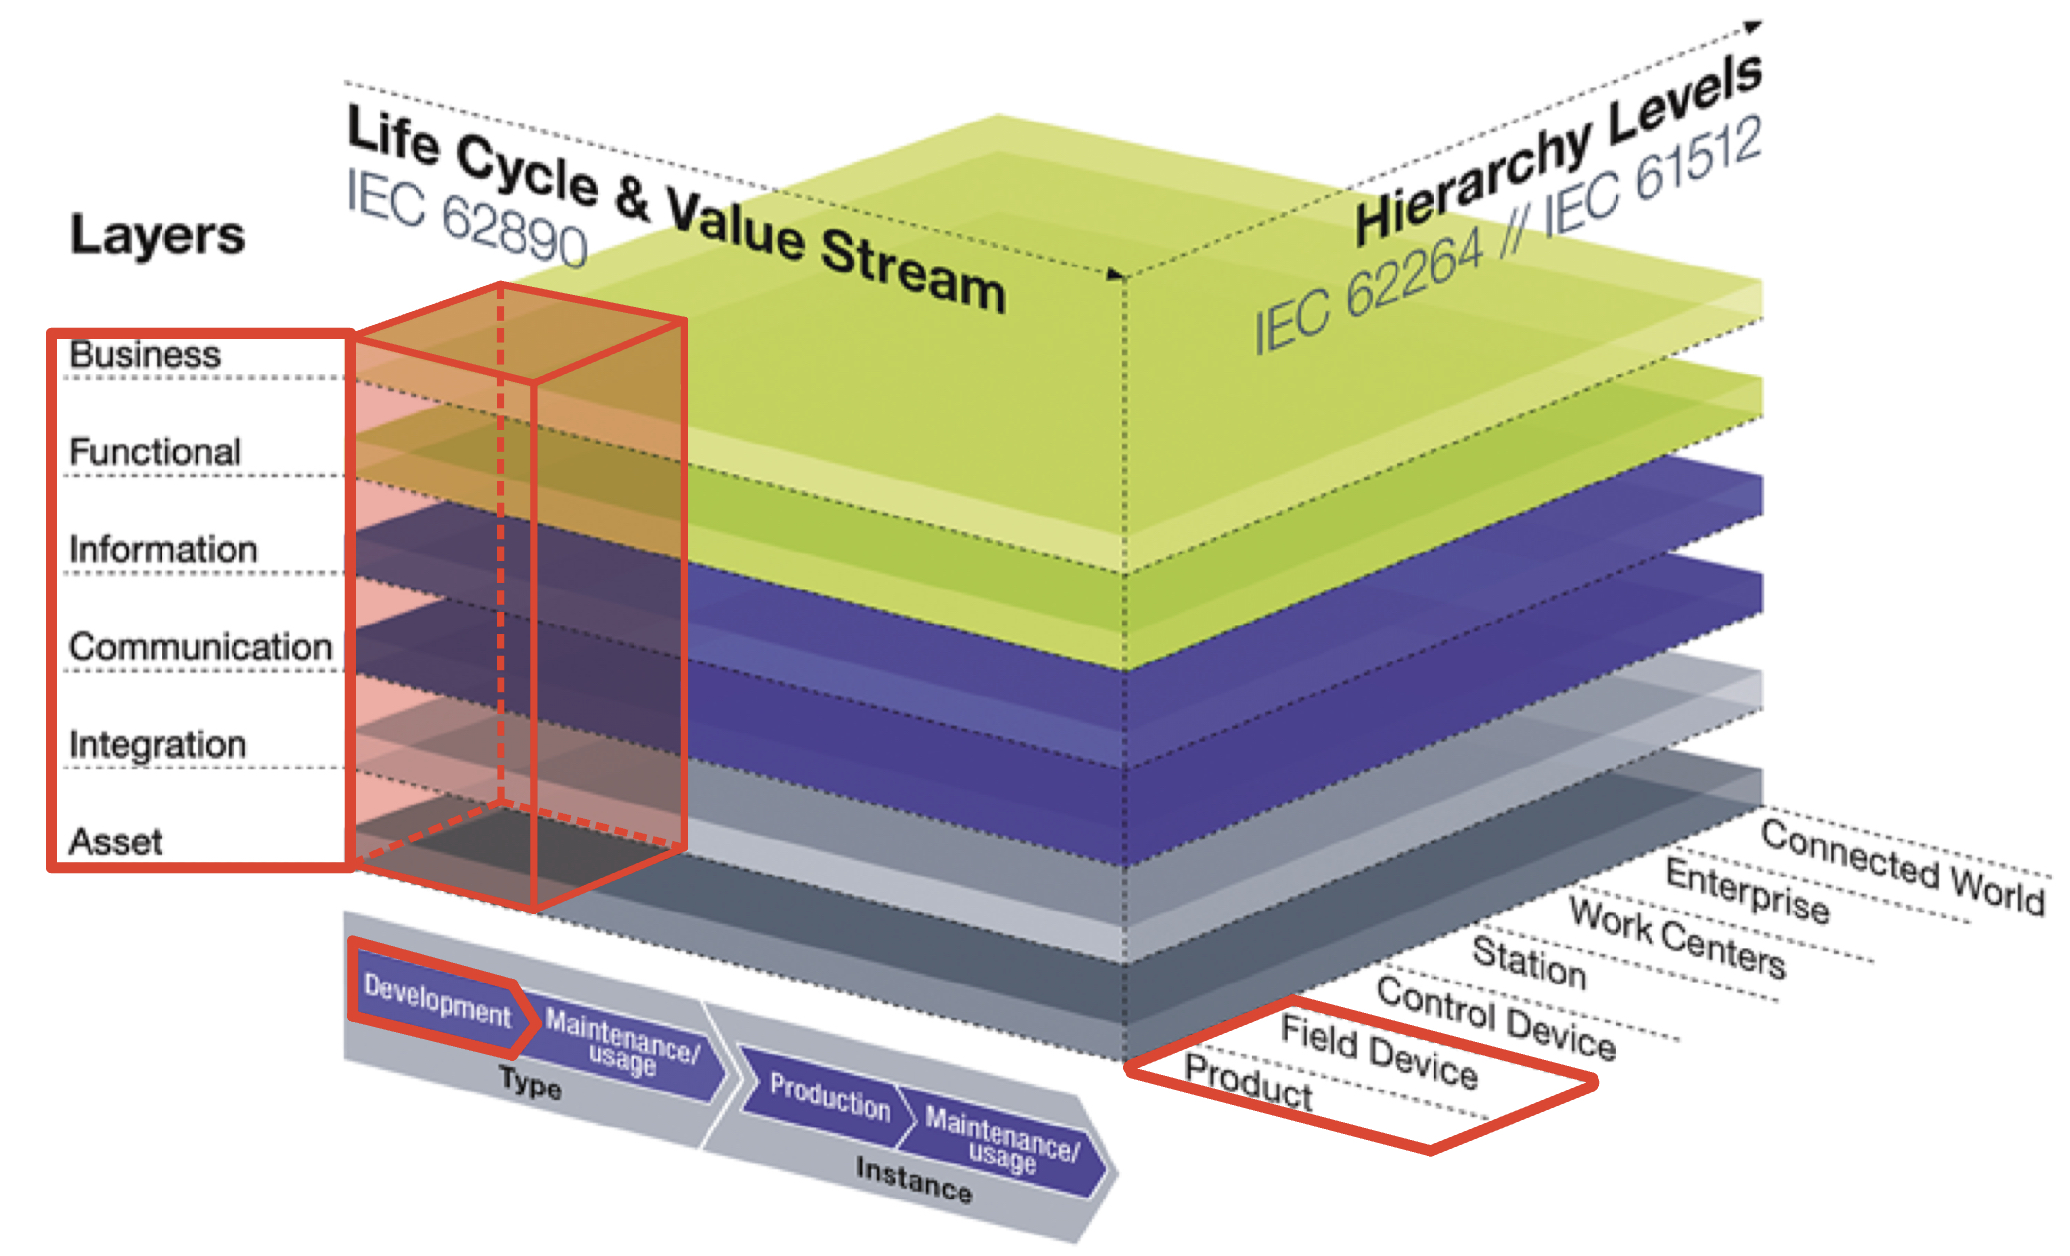
\includegraphics[scale=0.125]{img/Position of Analytic Application in RAMI4.jpg}
    \caption{Position of Analytic Application in RAMI 4.0 based on: \cite{Hankel2015}}
    \label{fig:Position of Analytic Application in RAMI 4.0}
\end{figure}
}

\section{Major requirement within the Infrastructure}
\STANDARD{\insertsection}
{
\textbf{1. Structural Requirement.}
\begin{itemize}
    \item   i. Closed Environment.
    \item  ii. Sensing device (Arduino Portenta H7 IMU).
    \item iii. Processing device.
    \item  iv. Power source (Li-Po battery 3.7V).   
\end{itemize}
\bigskip

\textbf{2. Technological requirements.}\\
\bigskip
\textbf{3. Scenario.}
}

\section{KDD Process}
\subsection{Problem's description}
\STANDARD{\insertsection}
{
\framesubtitle{\insertsubsection}

A gait pattern recognition system aims to identify patterns in an individual's walk that may indicate an impending injury, using data from inertial measurement units (IMUs) and algorithms to analyze the gait cycle. Hence, the goal is to enable early detection and potentially reduce the likelihood and severity of injuries, included below injury's type based on Data Selection:

\bigskip

\framesubtitle{\insertsubsection}
 \begin{figure}[ht]
        \begin{minipage}[b]{0.22\linewidth}
            \centering
            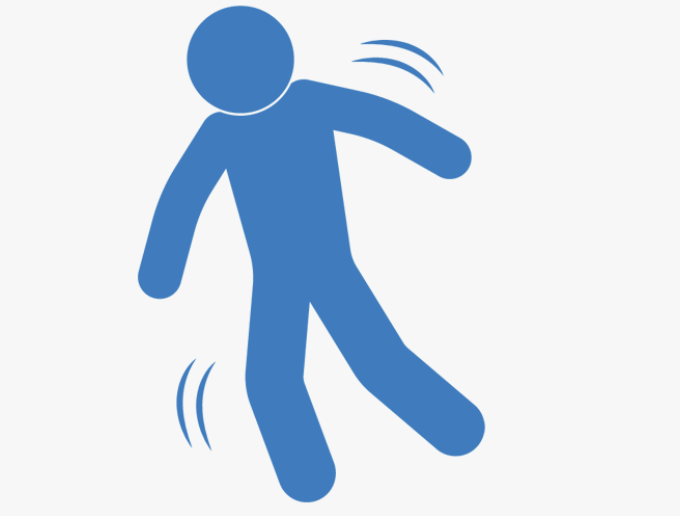
\includegraphics[width=\textwidth]{img/Balance Disorder.png}
            \caption{Balance Disorder source:\cite{BalanceDisorder2023}}
            \label{fig:a}
        \end{minipage}
        \hspace{0.5cm}
        \begin{minipage}[b]{0.20\linewidth}
            \centering
            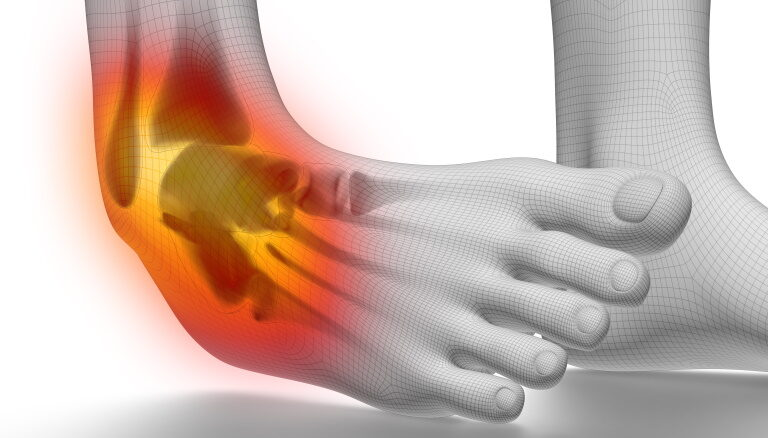
\includegraphics[width=\textwidth]{img/Ankle Sprain.jpeg}
            \caption{Ankle Sprain  source:\cite{AnkleSprain2023}}
            \label{fig:b}
        \end{minipage}
        \hspace{0.5cm}
         \begin{minipage}[b]{0.20\linewidth}
            \centering
            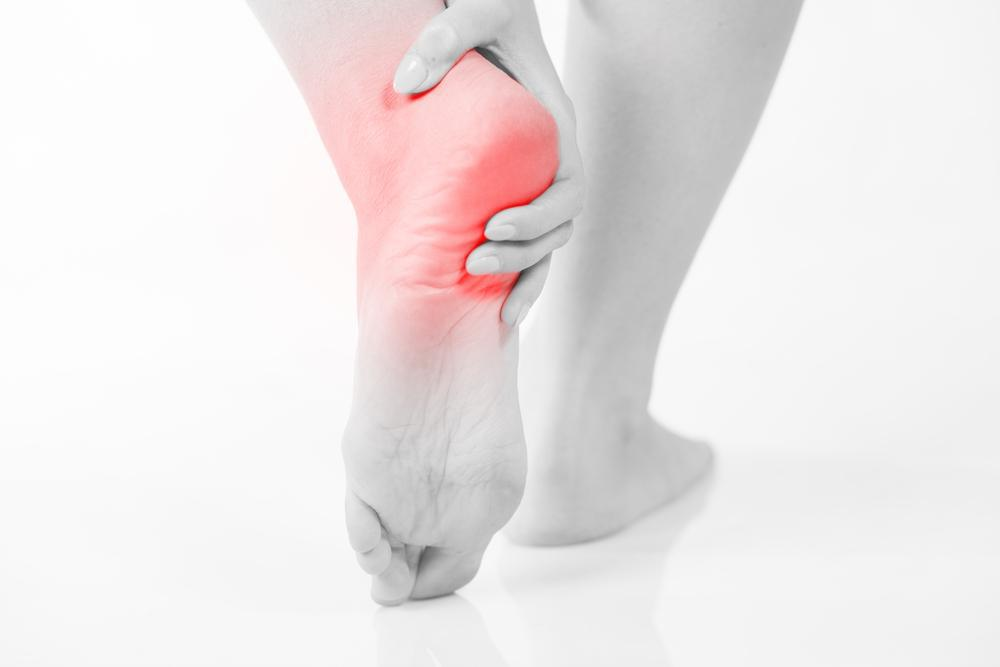
\includegraphics[width=\textwidth]{img/Plantar Fasciitis.jpeg}
            \caption{Plantar Fasciitis  source:\cite{PlantarFasciitis2023}}
            \label{fig:b}
        \end{minipage}
    \end{figure}
}


\subsection{Database}
\STANDARD{\insertsection}
{
\framesubtitle{\insertsubsection}

Acceleration signals along the three axes and timing data are measured in seconds and meters per second, respectively, for each gait phase. Three parameters can be used to evaluate the amount of data for a single research participant as follow:
\begin{equation}
\label{eqn:2.1}
    Total\:Data = N_{Step} \times N_{Gait} \times N_{Axis}
\end{equation}
where: \\

$N_{Step}$ = Number of given step, given by 1,408 base on: \cite{Hoeger2008}\\
\bigskip

$N_{Gait}$ = Number of Gait Phase Data set (HS, TS, HO, TO), given by 4.\\
\bigskip

$N_{Axis}$ = Number of axis for each gait phase (X, Y, Z), given by 6.\\
}

\subsection{Data Selection - Selection of Specific Gait Pattern}
\STANDARD{\insertsection}
{
\framesubtitle{\insertsubsection}
First, once we have the raw data, we can divide steps by the same foot by looking at the flat phases of $\ddot{z}_h$ and $\ddot{z}_t$, or by checking the periods where one of them is 0, meaning the heel or toe is touching the ground, defining heel flat phase or toe flat phase

\begin{figure}[ht]
    \centering
    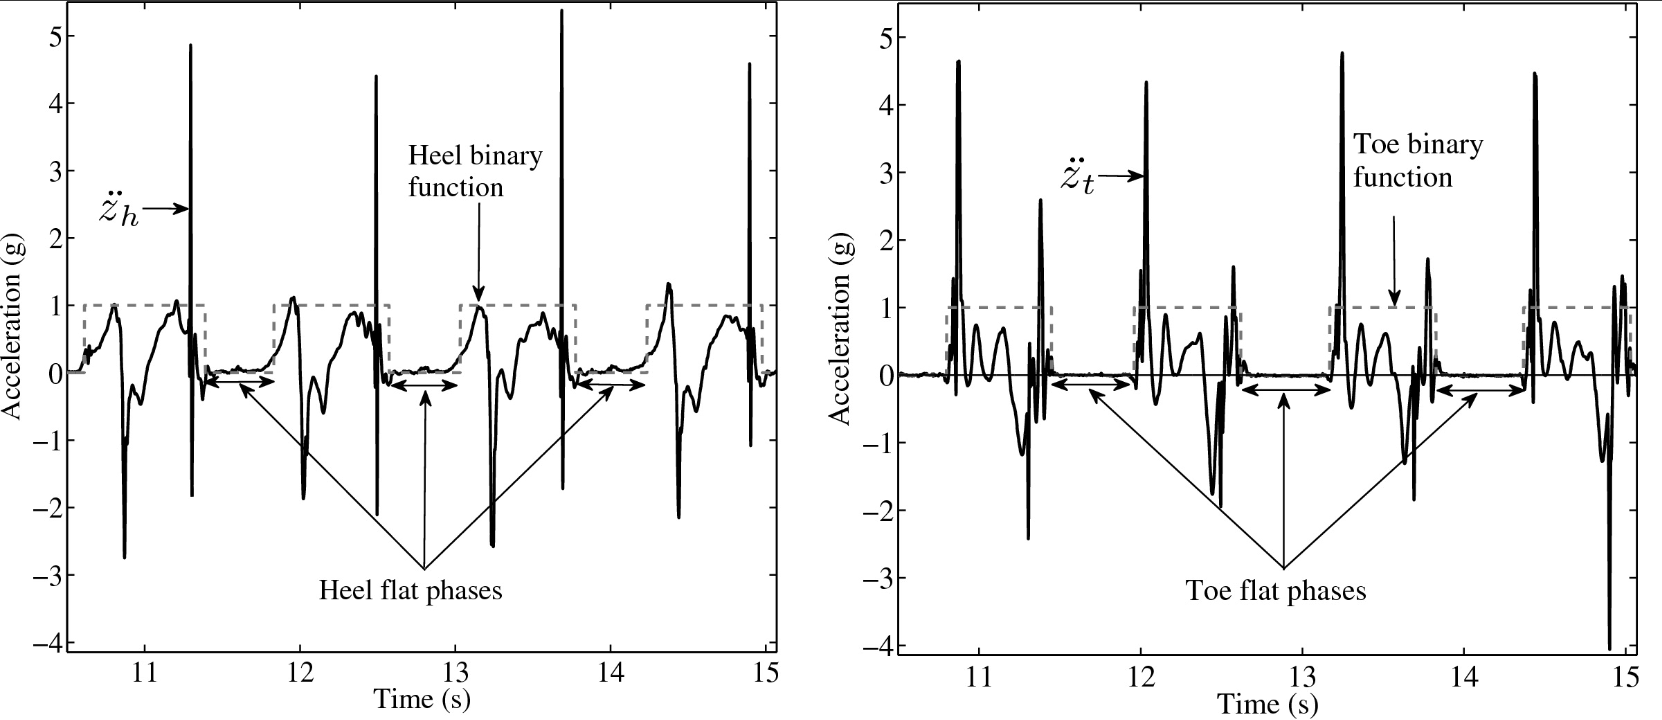
\includegraphics[scale=0.15]{img/flat-phases.png}
    \caption{Flat phases represented by $\ddot{z}_h$ and $\ddot{z}_t$ respectively based on: \cite{Mohamed2015}}
    \label{fig:Flat phases represented by heel flat phase or toe flat phase}
\end{figure}
}

\subsection{Data Preparetion - Gait Extraction}
\STANDARD{\insertsection}
{
\framesubtitle{\insertsubsection}
Gait cycle extraction will prepare the data for RNN (RNN). The binary functions representing the heel and toe are produced at this time scale. Using the local information associated with flat phase boundaries, our method uses the Butterworth filter to extract the four gait events of interest from accelerometer motion intervals. Which can be defined as follow.
\begin{itemize}
    \item a. Heel Strike (HS)
    \item b. Toe Strike (TS)
    \item c. Heel-Off (HO)
    \item d. Toe-Off (TO)
\end{itemize}
}

\subsection{Data Transformation - Data Mapping}
\STANDARD{\insertsection}
{
\framesubtitle{\insertsubsection}
\begin{table}[h!]
\centering
\resizebox{3cm}{!}{
\begin{tabular}{ | m{6em} | m{2.6cm}|} 
  \hline
  \multicolumn{2}{|c|}{$Data$}\\
  \hline
  $Parameter$ & $Unit$ \\ 
  \hline
  \hline
  \multicolumn{2}{|c|}{$Person ID$}\\
  \hline
  Weight \newline Height \newline Age & kg \newline m \newline years \\ 
  \hline
  \multicolumn{2}{|c|}{$Gait\:Phase\:Mean$}\\
  \hline
  $HS_{mean}$ $TS_{mean}$ $HO_{mean}$  $TO_{mean}$  & \{s, s\} \\ 
  \hline
  \multicolumn{2}{|c|}{$Velocity\:Xaxis\:Mean$}\\
  \hline
  $V_{HS_{Xmean}}$ $V_{TS_{Xmean}}$ $V_{HO_{Xmean}}$  $V_{TO_{Xmean}}$ & \{m/s, m/s\} \\ 
  \hline
  \multicolumn{2}{|c|}{$Velocity\:Yaxis\:Mean$}\\
  \hline
  $V_{HS_{Ymean}}$ $V_{TS_{Ymean}}$ $V_{HO_{Ymean}}$  $V_{TO_{Ymean}}$ & \{m/s, m/s\} \\ 
  \hline
  \multicolumn{2}{|c|}{$Velocity\:Zaxis\:Mean$}\\
  \hline
  $V_{HS_{Zmean}}$ $V_{TS_{Zmean}}$ $V_{HO_{Zmean}}$  $V_{TO_{Zmean}}$ & \{m/s, m/s\} \\
  \hline
\end{tabular}}
\caption{Format of dataset for one research participant }
\label{table:Format of dataset for one research participant}
\end{table}
}

\subsection{Data Mining - Recurrent Neural Network (RNN)}
\STANDARD{\insertsection}
{
\framesubtitle{\insertsubsection}
We consider that a Recurrent Neural Network (RNN) is the most appropriate neural network type for our injury detection system.

\bigskip

About 100 individuals with each of the four output types (balance disorders, ankle sprain, plantar fasciitis, and normal gait) could be sufficient for a reliable prediction.

\bigskip

For training the algorithm, we divided the data set into two batches: one containing 80\% of the data and the other containing 20\%.

\bigskip

To determine the number of hidden layers in our algorithm, we must consider the size and complexity of the input data. Excessive additions can cause overfitness and slower training. Portenta H7 size must also be considered. Various quantities and sizes of layers must be tested to determine the optimal combination.
}

\subsection{Model - Summary diagram}
\STANDARD{\insertsection}
{
\framesubtitle{\insertsubsection}
\begin{figure}[ht]
    \centering
    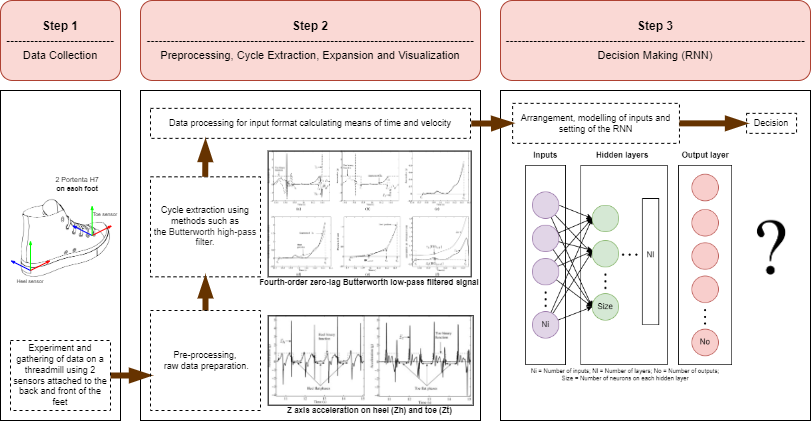
\includegraphics[scale=0.36]{img/Summary-diagram.png}
    \caption{Summary diagram}
    \label{fig:Summary diagram}
\end{figure}
}

\subsection{Validation \& Model in Production}
\STANDARD{\insertsection}
{
\framesubtitle{\insertsubsection}

\textbf{Validation}
To evaluate the performance of our RNN, we will use the sklearn library to test its accuracy on a 20\% sample of the labeled data. We may also validate the results using cross-validation or additional data sets. If the accuracy is low, we may need further adjustments, such as data normalization.

\bigskip

\textbf{Model in Production}
Our model is deployed in a real-world setting to predict injuries by analyzing measurements of people walking. The scalability of our method allows us to adjust the number of steps for increased reliability. The information is held in a secure environment, and the system is easy to maintain, as it only uses four sensors. If any malfunction occurs, it can be easily detected by an increase in outliers in the gait analysis phase.
}


\subsection{Conclusion}
\STANDARD{\insertsection}
{
\framesubtitle{\insertsubsection}
Our gait analysis system is more participant-friendly and requires fewer sensors than conventional methods. Finding the optimum number of steps for the neural network may involve physical analysis and testing with varying data volumes. We are also considering the feasibility of creating a fall detection neural network that could be integrated into Arduino devices to halt data collection and the treadmill in the event of a fall. In the grand scheme of things, this would be a great addition.
}